\documentclass[11pt,a4paper,twocolumn]{IEEEtran}
\usepackage[utf8]{inputenc}
\usepackage{tabularx, booktabs}
\usepackage{amsmath}
\usepackage{amsfonts}
\usepackage{caption}
\usepackage{pdfpages}
\usepackage[margin=2.5cm]{geometry}
\usepackage{listings}
\usepackage{amssymb}
\usepackage{hyperref}
\usepackage{graphicx}
\usepackage{svg}

\usepackage{biblatex}
\addbibresource{bib3.bib}

\newcolumntype{L}[1]{>{\raggedright\let\newline\\\arraybackslash\hspace{0pt}}m{#1}}
\newcolumntype{C}[1]{>{\centering\let\newline\\\arraybackslash\hspace{0pt}}m{#1}}
\newcolumntype{R}[1]{>{\raggedleft\let\newline\\\arraybackslash\hspace{0pt}}m{#1}}

% \sepline dopo \maketitle rende tutto più carino
\newcommand{\sepline}{\noindent\makebox[\linewidth]{\rule{\textwidth}{1.2pt}}}
\newcommand{\bsepline}{\noindent\makebox[\linewidth]{\rule{7.5cm}{1.2pt}}}
%\newcommand{\esepline}{\noindent\makebox[\linewidth]{\rule{7.5cm}{0.5pt}}}
\newcommand{\thinsepline}{\noindent\makebox[\linewidth]{\rule{7.5cm}{0.02pt}}}
\newcommand{\thinnersepline}{\noindent\makebox[\linewidth]{\rule{7.5cm}{0.01pt}}}

\author{Monaco Saverio - 2012264 \sepline \\Neural Networks and Deep Learning - Professor: A. Testolin}
\title{{\normalsize\textsc{Università degli studi di Padova}}\vspace{-.5cm} \\ \sepline\\ \textbf{Homework \#3
\\ Deep Reinforcement Learning}}

\begin{document}
	\maketitle
	\begin{abstract} The final homework concerns Deep-Q Learning, an algorithm of Deep Reinforcement Learning based on \textit{Bellman equation} for decision processes.\\
	Two environments of OpenAI Gym are tested with the Deep-Q Learning algorithm: "CartPole-v1" where a 2-dimensional platform must balance straight a pole, and a custom environment of a popular mobile game "FlappyBird".\\
	For the latter, two different state-space encodings are probed, a smaller state that employ 2 distances variable, and a bigger one that represent the game visual output.
	\end{abstract}
    \section*{\textbf{Deep-Q Learning}}
    Deep-Q Learning algorithm belongs to the class of Deep Learning problems of Reinforcement Learning.
    In this branch of Deep Learning, an agent can interact with the surrounding environment (simulated or real). By the resulting environment it is possible to give the agent a reward, namely a parameter that it tries to maximize.\\
    The goal of this algorithm is to find an optimal \textit{policy}, namely a rule that tells what action to make, given the state of the system. The way to determine the \textit{policy function} is not unique, Deep-Q Learning relies on \textit{Bellman equation} with the hypothesis that every instance is a Markov Process.\medskip\\
    For both environments, two optimizations are implemented to the vanilla algorithm:
    \begin{itemize}
		\item \textit{Experience Replay:} The agent does not learn while it acts on the environment. It follows the last policy for an arbitrary number of episodes, then it updates its policy sampling from its past [state, action] pairs. This helps the convergence of the algorithm by having a more i.i.d like data samples.
		\item \textit{Target Network:} Two similar networks are implemented for a more stable update rule
	\end{itemize}
	% explain deep q learning
	\section{\textbf{CartPole-v1}}
		% explain game
		\begin{figure}[h]
			\centering
			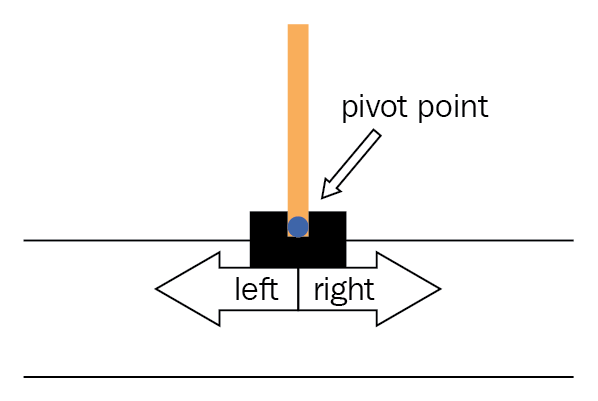
\includegraphics[width=0.75\linewidth]{../imgs/cartpole}
			\caption{CartPole-v1 graphical representation}
		\end{figure}
		\subsection{\textbf{Methods}}
		% describe your model architectures and hyperparameters
		\subsection{\textbf{Results}}
		%  present the simulation results
		
	% explain deep q learning
	\section{\textbf{FlappyBird}}
		% explain game
		\subsection{\textbf{FlappyBird-v0}}
			\subsubsection{\textbf{Methods}}
			% describe your model architectures and hyperparameters
			The state space are the two parameters of this environment, namely:
			\begin{itemize}
				\item horizontal distance to the next pipe:\\ range = [-$\infty$,+$\infty$]
				\item difference between the player's y position and the next hole's y position:\\ range = [-$\infty$,+$\infty$]
			\end{itemize}
			While the possible actions are just two:
			\begin{itemize}
				\item Fly upwards (originally the tap of the screen): \texttt{action value = 1}
				\item Do nothing \texttt{action value = 0}
			\end{itemize}
		
			\begin{figure}[h]
				\centering
				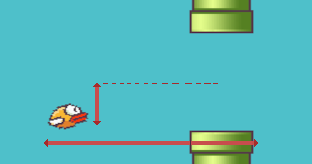
\includegraphics[width=0.75\linewidth]{../imgs/github1}
				\caption{State space of FlappyBird-v0 environment}
			\end{figure}
			Regarding the reward and punishes, the agent takes a point for every frame it is alive, and it gets a punishment proportionally to the vertical distance of the next hole.\medskip\\
		
			Being highly similar to the last environment, it was built another network class called just \texttt{Flappy} with only some minor tweaks to the class already built.
			Likewise the last task, the hyperparameters were tuned using Optuna:
			\thinsepline\\
			\textbf{Parameters for Optuna Optimization:}\medskip\\
			\begin{tabular}{ll}
				Trials: & \\
				Epochs: & \\
				\hline\\
				Lr: & \\
				Optimizer: & \\
				Gamma: & \\
				Initial T:& \\
			\end{tabular}\\
			\thinsepline\\
			During the parameter optimizations, the policies of the model were tested every 10 episodes (at T=0) to check if it already learned how to properly play. The criterion for a policy to be satisfying is to get a mean score greater than ??? over 10 games.
			\subsubsection{\textbf{Results}}\text{   }\\
			%  present the simulation results
			\thinsepline\\
			\textbf{Best parameters:}\medskip\\
			\begin{tabular}{ll}
				Learned in: & ??? epochs\\
				\hline\\
				Lr: & \\
				Optimizer: & \\
				Gamma: & \\
				Initial T:& \\
			\end{tabular}\\
			\thinsepline\\
		\subsection{\textbf{FlappyBird-rgb-v0}}
			\subsubsection{\textbf{Methods}}
			% describe your model architectures and hyperparameters
			\subsubsection{\textbf{Results}}
			%  present the simulation results
		
	\section{\textbf{Conclusions}}
	
	\newpage
	a
	\newpage
	\onecolumn
	\section{\textbf{Appendix}}
\end{document}